\section{Performance Benchmark}
\label{chp:performance}
All the benchmark test suites are run on a machine with AMD Ryzen 7 5800X3D 8-Core Processor, one GeForce RTX 4090 graphic card and 32G * 4 DDR4 ram.

During the execution of \zkwasm, there exist four different costs, namely the simulation cost, the synthesize cost, the proof generation cost (for separated code segments), and the proof batching cost. The simulation cost is the time needed for the WASM simulator to run the program. This is usually comparable with a standard WASM interpreter like wasmi and is slow then an optimized WASM runtime like wasmtime. Ingeneral the simulation process is hard to parallel. The synthesize cost is used to generate the witness table for the \zkwasm\, circuit. The proving generation cost is the most significant time consuming part the \zkwasm, which generates the proof of the execution of a single code segment. If the size of the execution trace of a program does not fit into a single code segment (more than $2^{24}$ instructions), then we need to split the execution trace into multiple segments and batching the proof of each segments which introduce the batching cost.

\subsection{Benchmark for single segment}
Unlike a traditional VM, in which, instructions might have different execution time, the main cost of the \zkwasm, is the evaluation of each polynomial (represent by the column of the witness table). Recall that in zkWASM each instruction occupies 4 rows in the witness table, thus the total proof generation time for each instruction is the same. With our loss of generality, we set the total rows of our circuit size to be $2^{20}$, $2^{19}$ and $2^{22}$ which theoretically can support the maximum trace of the $2^{18}$, $2^{19}$ and $2^{20}$ instructions. The sample programs we run with this setup include simple functions (Fibonacci and binary search), hash functions (SHA256 hash, keccak256), general purpose functions (JSON decoder/encoder, Syntax parser), etc.  


\begin{table}[!h]
\small
\begin{center}
\caption{Benchmark for Fibonacci \& binary search in \zkwasm}
\label{tbl:fib}
\begin{tabular}{ | c | c | c | c | c| c| }
  \hline
  circuit size & max trace size & max synthesize time & proof time & verify time \\ 
  \hline
  $2^{18}$ & 53677 & 0.2s & 4.8s & 22ms \\
  \hline
  $2^{19}$ & 108317 & 0.6s & 10s & 24ms \\
  \hline
    $2^{20}$ & 162033 & 1.2s & 20s & 22ms \\
  \hline
    $2^{21}$ & 462349 & 2.2s & 41s & 22ms \\
  \hline
    $2^{22}$ & 940346 & 4.5s & 82s & 29ms \\
  \hline
\end{tabular}

\end{center}
\end{table}
\begin{table}[!h]
\small
\begin{center}
\caption{Benchmark for hash functions in \zkwasm}
\label{tbl:hash}
\begin{tabular}{ | c | c | c | c | c| c| }
  \hline
  circuit size & max trace size & max synthesize time & proof time & verify time \\ 
  \hline
  $2^{18}$ & 49076 & 0.19s & 4.9s & 22ms \\
  \hline
  $2^{19}$ & 110259 & 0.6s & 10s & 24ms \\
  \hline
    $2^{20}$ & 150084 & 0.9s & 20s & 22ms \\
  \hline
    $2^{21}$ & 440737 & 2.2s & 41s & 22ms \\
  \hline
    $2^{22}$ & 862349 & 4 s & 84s & 29ms \\
  \hline
\end{tabular}
\end{center}
\end{table}

\begin{table}[!h]
\small
\begin{center}
\caption{Benchmark for general purpose functions in \zkwasm}
\label{tbl:general-purpose}
\begin{tabular}{ | c | c | c | c | c| c| }
  \hline
  circuit size & max trace size & max synthesize time & proof time & verify time \\ 
  \hline
  $2^{18}$ & 63134 & 0.22s & 4.9s & 22ms \\
  \hline
  $2^{19}$ & 109368 & 0.6s & 10s & 24ms \\
  \hline
    $2^{20}$ & 240523 & 1.2s & 20s & 22ms \\
  \hline
    $2^{21}$ & 420426 & 2.1s & 40s & 22ms \\
  \hline
    $2^{22}$ & 970862 & 4.6s & 84s & 29ms \\
  \hline
\end{tabular}
\end{center}
\end{table}

In Table [\ref{tbl:fib}, \ref{tbl:hash}, \ref{tbl:general-purpose}], the total number of rows of the witness table in \zkwasm\, as a power of two. The trace size denotes the total instructions included in the execution trace. The synthesize time is the time to generate all the witness needed and proof time is the time \zkwasm\, used to create the proof for the valid execution and the verify time is the time for a verifier to check the proof. From these data, we see that the verifying time is O(1) and the proof time grows linearly when the size of the circuit grows. The synthesize time describes the cost of the witness generation time which grows lineally as the trace size grows.
\subsection{Performance for Large Program with Proof Batching}
For a program with a large execution sequence, then the overall proving time will be the segment proving time plus the batching time. Similar to the \zkwasm\, circuit, the batching circuit (see Section \ref{chp:sharding-batching}) has its size limit as well. Thus in general, we can not batch all the segment in one round. In practical, we using the following batching pipeline.
\begin{figure}[!ht]
\centerline{
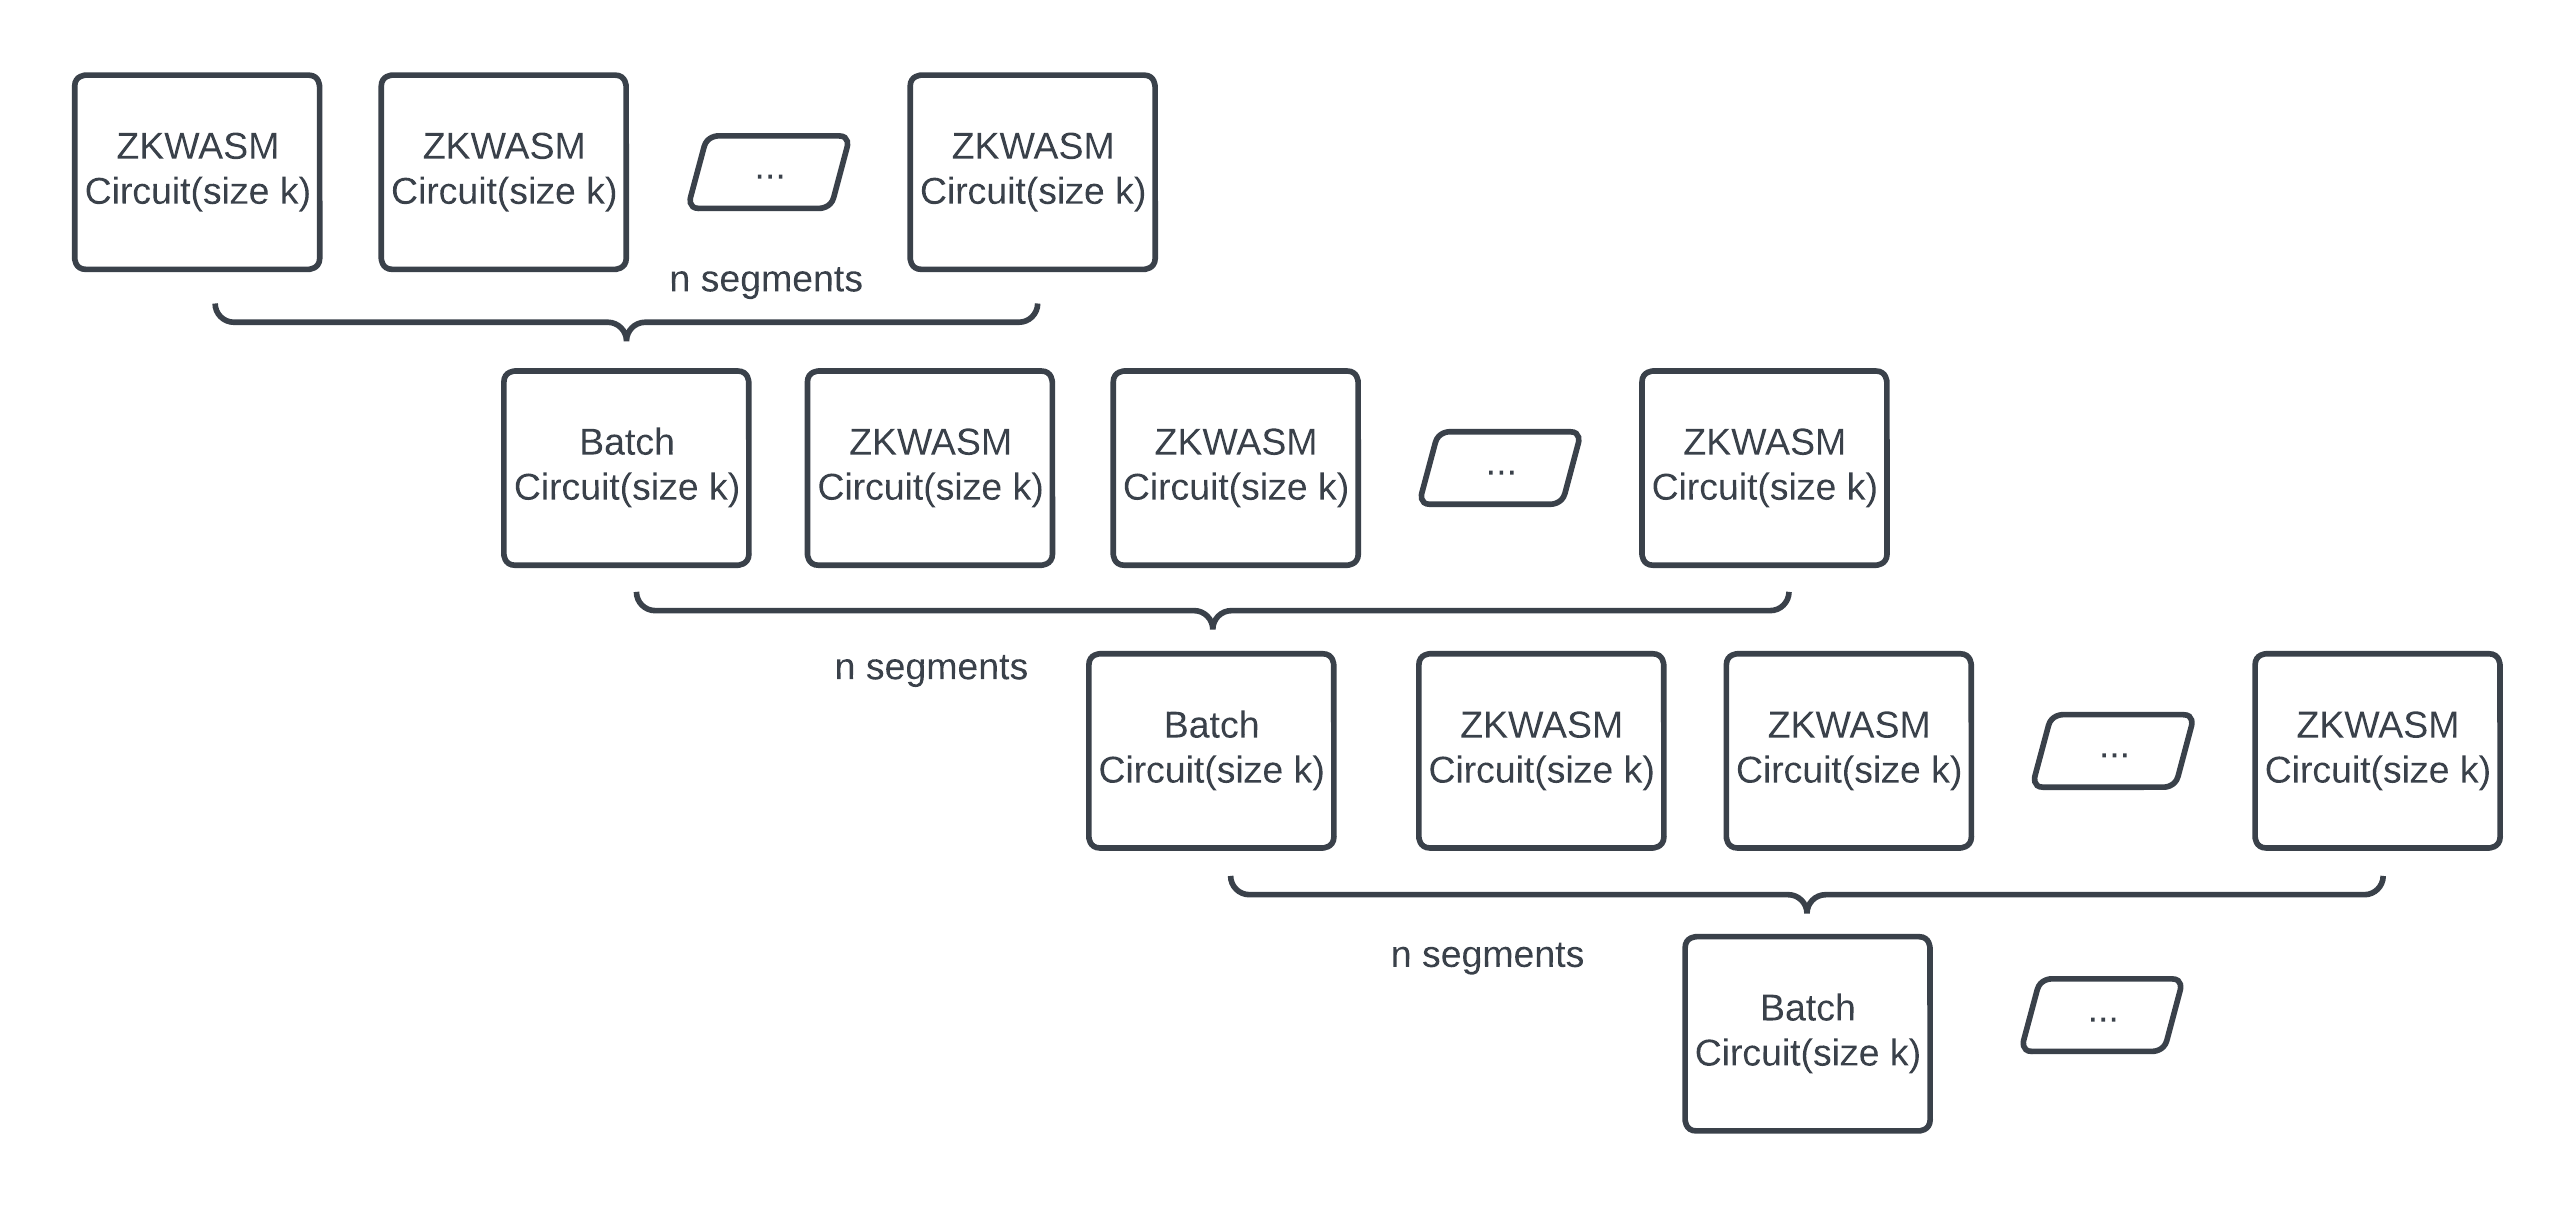
\includegraphics[scale=0.6]{figs/batch-pipeline.png}
}
\caption{Split execution sequence into sub sequence}
\label{fig:batch-pipeline}
\end{figure}

Based on the above pipeline, we would like to pick parameter $k$ and $n$ to maximize the overall performance (instruction per second). The table \ref{tbl:proof-batching} shows the relationship before $n$ and $k$ and the overall proving time for the batch circuit. 
\begin{table}[!h]
\small
\begin{center}
\caption{Benchmark for proof batching in \zkwasm}
\label{tbl:proof-batching}
\begin{tabular}{ | c | c | c | c | c | c | c| }
  \hline
  circuit size $k$ & code segment $n$ & proving time & verify time \\ 
  \hline
  $2^{21}$ & 1 & 23s & 4.7ms\\
  \hline
  $2^{22}$ & 2 & 46s & 4.63ms\\
  \hline
  $2^{23}$ & 4 & 95s & 4.77ms\\
  \hline
  $2^{24}$ & 8 & 192s & 5.05ms\\
  \hline
\end{tabular}
\end{center}
\end{table}
In conclusion, Both the number of segments can be batched and the proving time grows linearly as the circuit size of batch circuit. Thus he overall performance with circuit size $k$ can be abstracted as follows (where $ips$ denotes instructions per-second):
$$
 ips = \frac{k * n * t_{wasm} + k * t_{batch}}{k}
$$
By picking $k = 2^{24}$, we reach around $2^{15}$ instructions per-seconds when the program trace is large.

\section{Conclusion \& Further Work}
\label{chp:conclusion}
We presented \zkwasm, a WASM virtual machine that leverages the technology of \zksnark. As far as know, we are the first to present a novel way to implement the semantics of a WASM virtual machine in arithmetic circuits. Using \zkwasm, we are able to deploy serverless service in an untrusted cloud since \zkwasm\, does not only emulates the execution but also gives a correctness proof of the execution result. Hence any vulnerability on the cloud will not affect the correctness of the verifiable result (a faulty result cannot have correct ZKSNARK proof).

For large applications that provide large execution traces, we successfully applied the execution partition and proof batching technique so the \zkwasm\, scales when the program size grows. Regarding the performance, various optimization can be applied in the future including improving the commitment scheme \cite{chen2022hyperplonk}, adopting a better parallel computing strategy \cite{wu2018dizk}, using SNARK specific hardware \cite{peng2020design, xavier2022pipemsm}, etc.

